%package list
\documentclass{article}
\usepackage[top=3cm, bottom=3cm, outer=3cm, inner=3cm]{geometry}
\usepackage{multicol}
\usepackage{graphicx}
\usepackage{url}
%\usepackage{cite}
\usepackage{hyperref}
\usepackage{array}
%\usepackage{multicol}
\newcolumntype{x}[1]{>{\centering\arraybackslash\hspace{0pt}}p{#1}}
\usepackage{natbib}
\usepackage{pdfpages}
\usepackage{multirow}
\usepackage[utf8]{inputenc}
\usepackage[normalem]{ulem}
\useunder{\uline}{\ul}{}
\usepackage{svg}
\usepackage{xcolor}
\usepackage{listings}
\lstdefinestyle{ascii-tree}{
    literate={├}{|}1 {─}{--}1 {└}{+}1 
  }
\lstset{basicstyle=\ttfamily,
  showstringspaces=false,
  commentstyle=\color{red},
  keywordstyle=\color{blue}
}
%\usepackage{booktabs}
\usepackage{caption}
\usepackage{subcaption}
\usepackage{float}
\usepackage{array}

\newcolumntype{M}[1]{>{\centering\arraybackslash}m{#1}}
\newcolumntype{N}{@{}m{0pt}@{}}


%%%%%%%%%%%%%%%%%%%%%%%%%%%%%%%%%%%%%%%%%%%%%%%%%%%%%%%%%%%%%%%%%%%%%%%%%%%%
%CREACIÓN DE VARIABLE
\newcommand{\itemEmail}{jcondoripin@unsa.edu.pe}
\newcommand{\itemStudent}{Juan José Condori Pinto}
\newcommand{\itemCourse}{Programación Web 2}
\newcommand{\itemCourseCode}{1702122}
\newcommand{\itemSemester}{III}
\newcommand{\itemUniversity}{Universidad Nacional de San Agustín de Arequipa}
\newcommand{\itemFaculty}{Facultad de Ingeniería de Producción y Servicios}
\newcommand{\itemDepartment}{Departamento Académico de Ingeniería de Sistemas e Informática}
\newcommand{\itemSchool}{Escuela Profesional de Ingeniería de Sistemas}


%AQUIIII: CAMBIA LA INFO DEL LAB
\newcommand{\itemAcademic}{2023 - A}
\newcommand{\itemInput}{Del 04 de Julio 2023}
\newcommand{\itemOutput}{Al 14 de Julio 2023}
\newcommand{\itemPracticeNumber}{07}
\newcommand{\itemTheme}{Django - Relaciones uno a muchos y muchos a muchos en BD}
%%%%%%%%%%%%%%%%%%%%%%%%%%%%%%%%%%%%%%%%%%%%%%%%%%%%%%%%%%%%%%%%%%%%%%%%%%%%


%PARA EL PIE DE PÁGINA
\usepackage{fancyhdr}
\pagestyle{fancy}
\fancyhf{}
\setlength{\headheight}{30pt}
\renewcommand{\headrulewidth}{1pt}
\renewcommand{\footrulewidth}{1pt}
\fancyhead[L]{\raisebox{-0.2\height}{\includegraphics[width=3cm]{img/logo_episunsa.png}}}
\fancyhead[C]{\fontsize{7}{7}\selectfont	\itemUniversity \\ \itemFaculty \\ \itemDepartment \\ \itemSchool \\ \textbf{\itemCourse}}
\fancyhead[R]{\raisebox{-0.2\height}{\includegraphics[width=1.2cm]{img/logo_abet}}}
\fancyfoot[L]{Estudiante Juan José Condori Pinto}
\fancyfoot[C]{\itemCourse}
\fancyfoot[R]{Página \thepage}

% para el codigo fuente
\usepackage{listings}
\usepackage{color, colortbl}
\definecolor{dkgreen}{rgb}{0,0.6,0}
\definecolor{gray}{rgb}{0.5,0.5,0.5}
\definecolor{mauve}{rgb}{0.58,0,0.82}
\definecolor{codebackground}{rgb}{0.95, 0.95, 0.92}
\definecolor{tablebackground}{rgb}{0.8, 0, 0}

\lstset{frame=tb,
	language=bash,
	aboveskip=3mm,
	belowskip=3mm,
	showstringspaces=false,
	columns=flexible,
	basicstyle={\small\ttfamily},
	numbers=none,
	numberstyle=\tiny\color{gray},
	keywordstyle=\color{blue},
	commentstyle=\color{dkgreen},
	stringstyle=\color{mauve},
	breaklines=true,
	breakatwhitespace=true,
	tabsize=3,
	backgroundcolor= \color{codebackground},
}


\begin{document}
        %CARÁTULA
        \vspace*{10px}
    	
        \begin{center}	
            \fontsize{17}{17} \textbf{ Informe de Laboratorio \itemPracticeNumber}
        \end{center}
        \centerline{\textbf{\Large Tema: \itemTheme}}
        %\vspace*{0.5cm}	
    
        \begin{flushright}
    	\begin{tabular}{|M{2.5cm}|N|}
    		\hline 
    		\rowcolor{tablebackground}
    		\color{white} \textbf{Nota} \\
    		\hline 
    			\\[30pt]
    		\hline 			
    	\end{tabular}
        \end{flushright}	

	\begin{table}[H]
		\begin{tabular}{|x{4.7cm}|x{4.8cm}|x{4.8cm}|}
			\hline 
			\rowcolor{tablebackground}
			\color{white} \textbf{Estudiante} & \color{white}\textbf{Escuela}  & \color{white}\textbf{Asignatura}   \\
			\hline 
			{\itemStudent \par \itemEmail} & \itemSchool & {\itemCourse \par Semestre: \itemSemester \par Código: \itemCourseCode}     \\
			\hline 			
		\end{tabular}
	\end{table}		
	
	\begin{table}[H]
		\begin{tabular}{|x{4.7cm}|x{4.8cm}|x{4.8cm}|}
			\hline 
			\rowcolor{tablebackground}
			\color{white}\textbf{Laboratorio} & \color{white}\textbf{Tema}  & \color{white}\textbf{Duración}   \\
			\hline 
			\itemPracticeNumber & \itemTheme & 04 horas   \\
			\hline 
		\end{tabular}
	\end{table}
	
	\begin{table}[H]
		\begin{tabular}{|x{4.7cm}|x{4.8cm}|x{4.8cm}|}
			\hline 
			\rowcolor{tablebackground}
			\color{white}\textbf{Semestre académico} & \color{white}\textbf{Fecha de inicio}  & \color{white}\textbf{Fecha de entrega}   \\
			\hline 
			\itemAcademic & \itemInput &  \itemOutput  \\
			\hline 
		\end{tabular}
	\end{table}

\section{Temas a tratar}
        \begin{itemize}
            \item Proyectos de Django
            \item Aplicaciones en Django
            \item Relaciones uno a muchos en Django
            \item Relaciones de muchos a muchos en Django
            \item Django PDF y emails
        \end{itemize}
    
\section{Ejercicios}
\begin{itemize}
    \item Reproducir las actividades de los videos donde se trabajan: relaciones de uno a muchos, muchos a muchos, impresión de PDFs y envío de emails.
    \item Crear un video en Flipgrid.
\end{itemize} 

    Estructura inicial del proyecto
    \begin{figure}
        \centering
        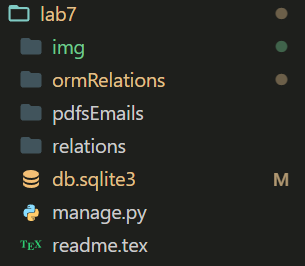
\includegraphics[width=150mm]{img/img0.png}
        \caption{Estructura inicial}
        \label{fig:enter-label}
    \end{figure}
    \begin{figure}
        \centering
        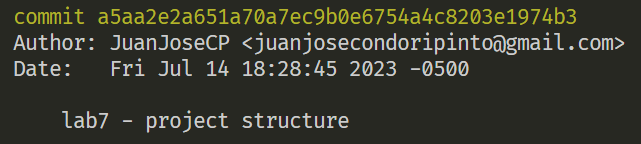
\includegraphics[width=150mm]{img/commit1.png}
        \caption{Commit de estructura inicial}
        \label{fig:enter-label}
    \end{figure}
    
    \subsection{Resolucion de ejercicios}
        \begin{figure}
            \centering
            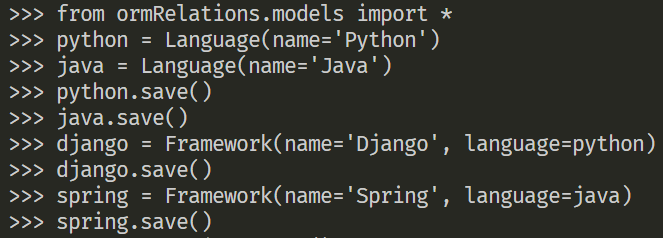
\includegraphics[width=150mm]{img/img1.png}
            \caption{Creacion de objetos y relacion de uno a muchos}
            \label{fig:enter-label}
        \end{figure}
        \begin{figure}
            \centering
            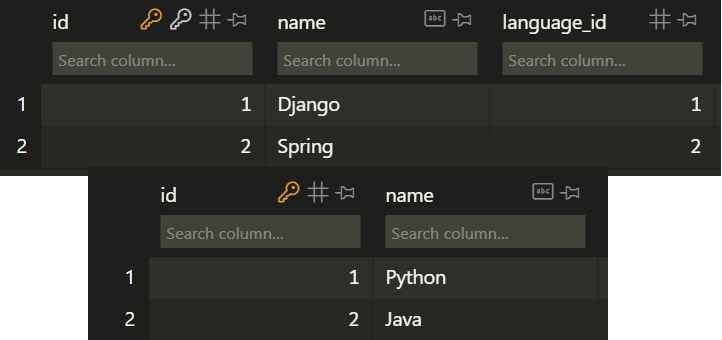
\includegraphics[width=150mm]{img/img2.png}
            \caption{Tablas creadas}
            \label{fig:enter-label}
        \end{figure}
        \begin{figure}
            \centering
            
\includegraphics[width=150mm]{img/img3.png}
            \caption{Relacion muchos a muchos}
            \label{fig:enter-label}
        \end{figure}
        \begin{figure}
            \centering
            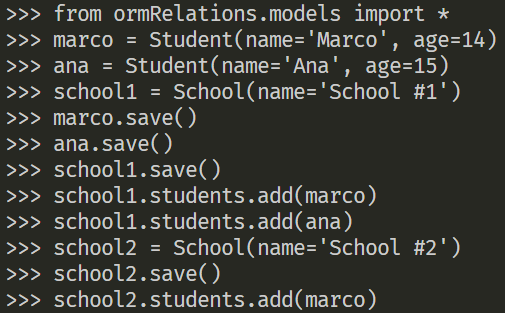
\includegraphics[width=150mm]{img/img4.png}
            \caption{Prueba con objetos iniciales}
            \label{fig:enter-label}
        \end{figure}
        \begin{figure}
            \centering
            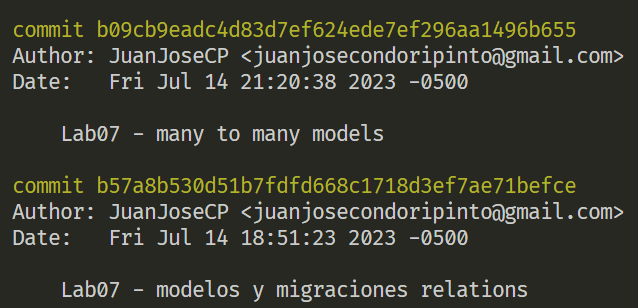
\includegraphics[width=150mm]{img/commit2.png}
            \caption{Commit de creacion de tablas y migraciones}
            \label{fig:enter-label}
        \end{figure}
        \begin{figure}
            \centering
            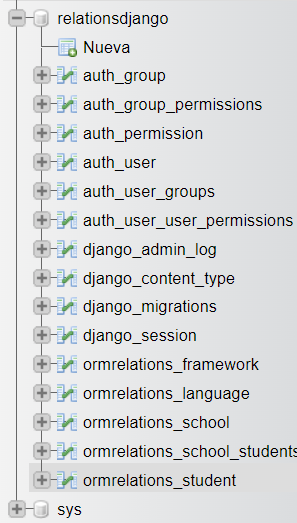
\includegraphics[width=150mm]{img/img5.png}
            \caption{Base de datos creada en phpmyadmin}
            \label{fig:enter-label}
        \end{figure}
        \begin{figure}
            \centering
            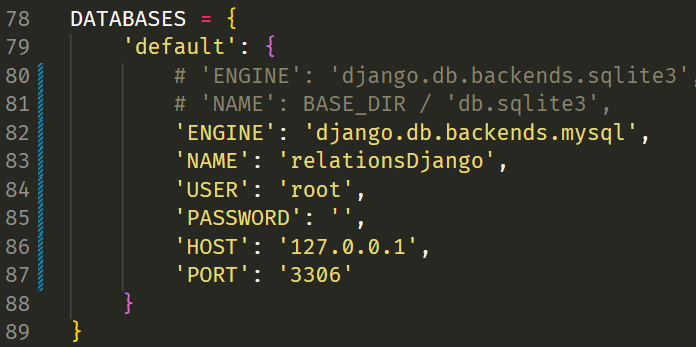
\includegraphics[width=150mm]{img/img6.png}
            \caption{Configuracion de conexion con nueva base de datos}
            \label{fig:enter-label}
        \end{figure}
        \begin{figure}
            \centering
            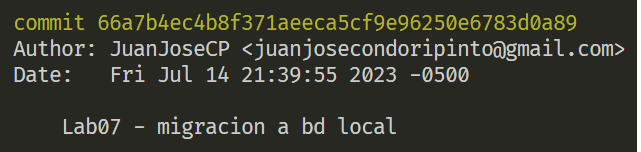
\includegraphics[width=150mm]{img/commit3.png}
            \caption{Commit de migracion a base de datos local}
            \label{fig:enter-label}
        \end{figure}
        \begin{figure}
            \centering
            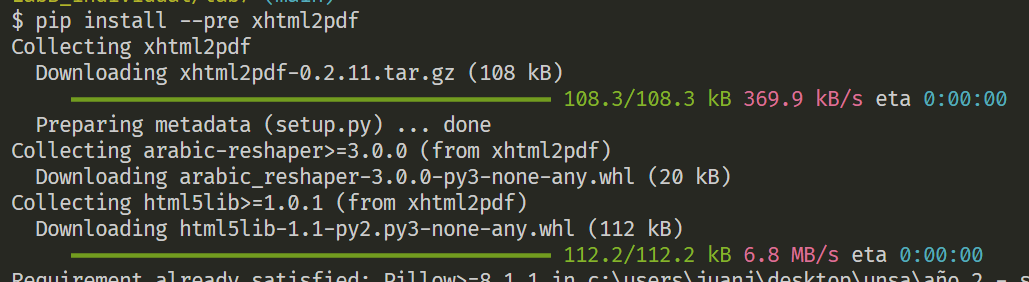
\includegraphics[width=150mm]{img/img7.png}
            \caption{Instalacion de paquete para impresion de pdf}
            \label{fig:enter-label}
        \end{figure}
        \begin{figure}
            \centering
            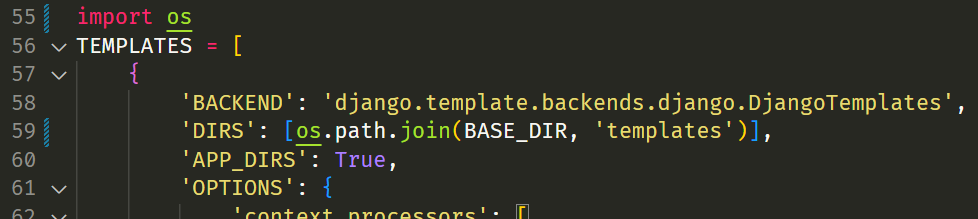
\includegraphics[width=150mm]{img/img8.png}
            \caption{Enlace con templates}
            \label{fig:enter-label}
        \end{figure}
        \begin{figure}
            \centering
            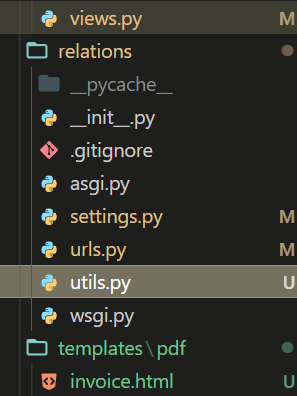
\includegraphics[width=150mm]{img/img9.png}
            \caption{Estructura de proyecto de pdf}
            \label{fig:enter-label}
        \end{figure}
        \begin{figure}
            \centering
            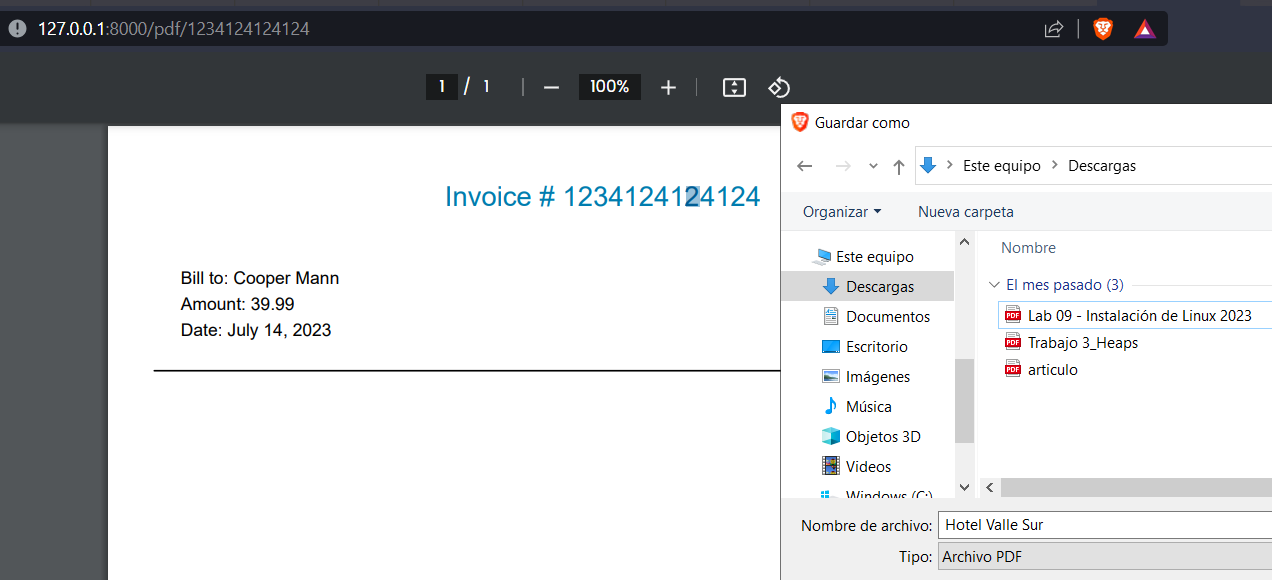
\includegraphics[width=150mm]{img/img10.png}
            \caption{Vista index de template pdf de ejemplo}
            \label{fig:enter-label}
        \end{figure}
        \begin{figure}
            \centering
            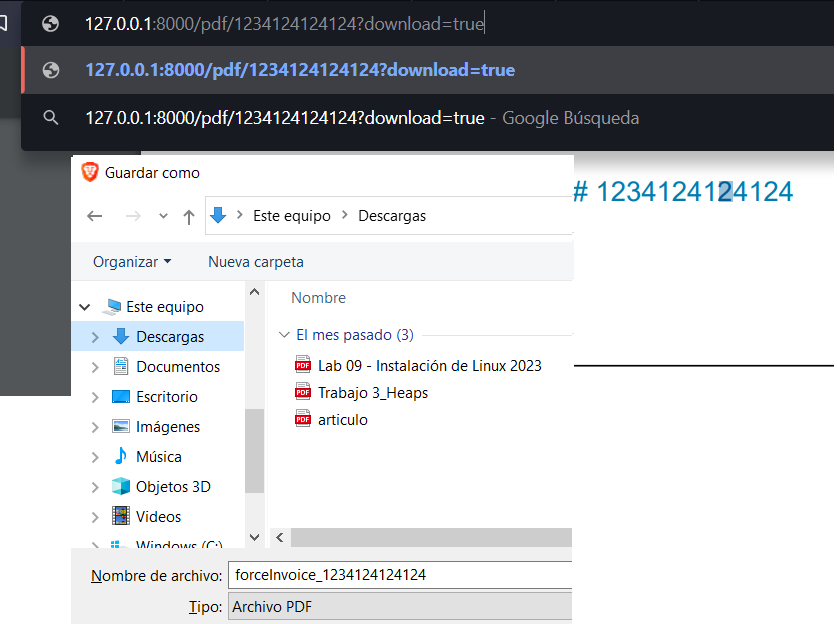
\includegraphics[width=150mm]{img/img11.png}
            \caption{Descarga forzada}
            \label{fig:enter-label}
        \end{figure}
        \begin{figure}
            \centering
            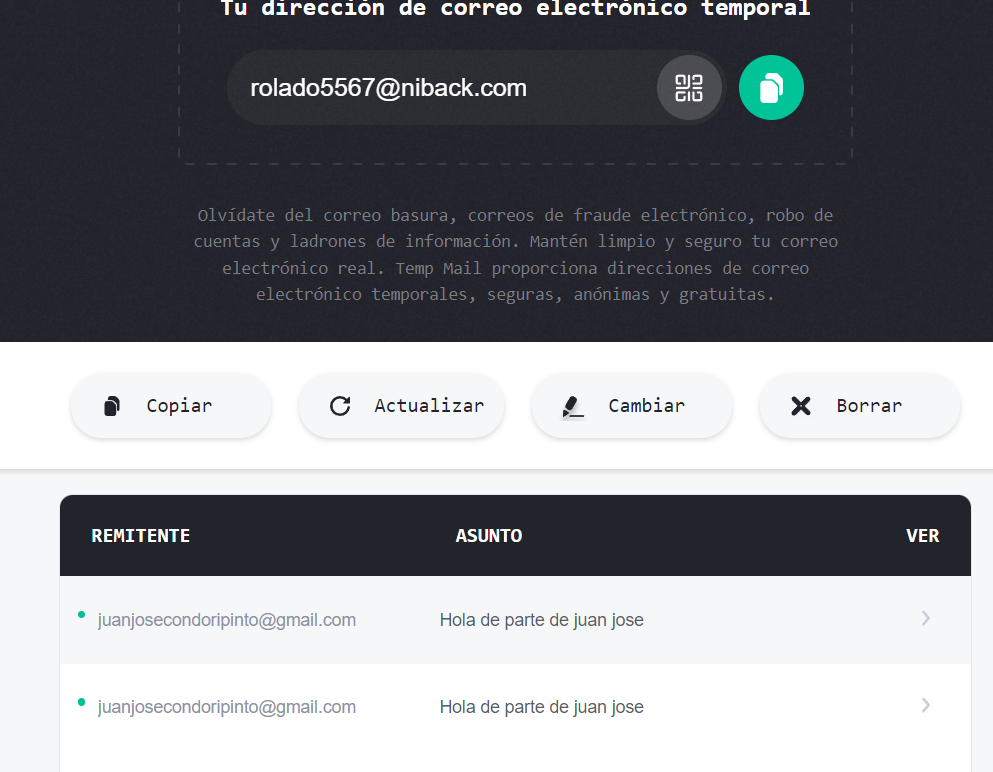
\includegraphics[width=150mm]{img/img12.png}
            \caption{Envio de email a correo falso}
            \label{fig:enter-label}
        \end{figure}
        \begin{figure}
            \centering
            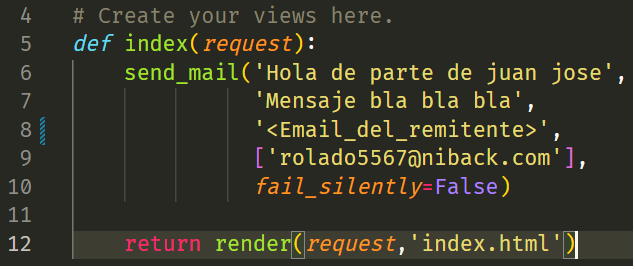
\includegraphics[width=150mm]{img/img13.png}
            \caption{View index con envio de email}
            \label{fig:enter-label}
        \end{figure}
        \begin{figure}
            \centering
            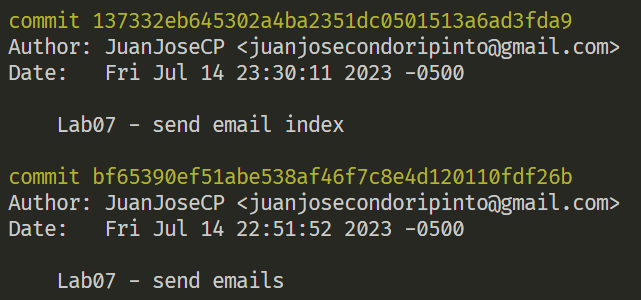
\includegraphics[width=150mm]{img/commit4.png}
            \caption{Commit para envio de emails a correos falsos}
            \label{fig:enter-label}
        \end{figure}
    \newpage
    \subsection{Videos}
        Parte 1: \href{https://flip.com/s/y4LkgKW_kXnS}{Part1}
        Parte 2: \href{https://flip.com/s/Zvr3Pnzpbx5_}{Part2}
        Parte 3: \href{https://flip.com/s/TssDry1NFsxz}{Part3}

\newpage
\section{\textcolor{red}{Rubricas}}
        \subsection{\textcolor{red}{Rubrica para entregable Informe}}
            \begin{table}[ht]
                \centering
                \caption{Rúbrica para tipo de informe}
                \begin{tabular}{
                        |p{2.5cm}
                        |p{6cm}
                        |p{2cm}
                        |p{2cm} |}
                    \hline
                        \multicolumn{2}{|c|}{\textbf{Informe}} & \centerline{\textbf{Cumple}} & \centerline{\textbf{No cumple}} \\
                    \hline
                        \textbf{\textcolor{red}{Latex}} & \textcolor{blue}{El informe esta en formato PDF desde Latex, con un formato limpio (buena presentación) y facil de leer.} & \centerline{20} & \centerline{0} \\
                    \hline
                        \textbf{MarkDown} & El informe esta en formato PDF desde MarkDown README.md, con un formato limpio (buena presentacion) y facil de leer. & \centerline{17} & \centerline{0}\\
                    \hline
                        \textbf{MS Word} & El informe esta en formato PDF desde plantilla MS Word, con un formato limpio (buena presentacion) y facil de leer. & \centerline{15} & \centerline{0}\\
                    \hline
                        \textbf{Observaciones} & Por cada observacion se le descontara puntos. & \centerline{-} & \centerline{-}\\
                    \hline
                    \end{tabular}
                \label{tab:tab1}
            \end{table}
            
        \subsection{\textcolor{red}{Rubrica para el contenido del Informe y demostracion}}
            \begin{itemize}
                \item El alumno debera marcar o dejar en blanco en las celdas de la columna Checklist, deacuerdo a si cumplio o no con el ́ıtem correspondiente.
                \item Si un alumno supera la fecha de entrega, su calificacion siempre sera sobre la nota mınima aprobada, siempre y cuando cumpla con todos lo items.
                \item El alumno debe autocalificarse en la columna Estudiante de acuerdo a la tabla de calificacion de niveles de desempeño:
            \end{itemize}
            \begin{table}[ht]
                \centering
                \caption{Niveles de desempeño}
                \begin{tabular}{
                        >{\centering\arraybackslash}m{1.2cm}
                        >{\centering\arraybackslash}m{3cm}
                        >{\centering\arraybackslash}m{3cm}
                        >{\centering\arraybackslash}m{3cm}
                        >{\centering\arraybackslash}m{3cm}}
                    \hline
                    \multicolumn{5}{c}{Nivel} \\
                    \hline
                    \textbf{Puntos} & Insatisfactorio 25\% & En Proceso 50\% & Satisfactorio 75\% & Sobresaliente 100\% \\
                    \textbf{2.0} & 0.5 & 1.0 & 1.5 & 2.0 \\
                    \textbf{4.0} & 1.0 & 2.0 & 3.0 & 4.0 \\
                    \hline
                \end{tabular}
                \label{tab:tab2}
            \end{table}
            \begin{table}[]
                \centering
                \caption{Rubrica para contenido del Informe y demostracion}
                \begin{tabular}{
                    |m{2.5cm}
                    |m{7cm}
                    |>{\centering\arraybackslash}m{1cm}
                    |>{\centering\arraybackslash}m{1.2cm}
                    |>{\centering\arraybackslash}m{1.5cm}
                    |>{\centering\arraybackslash}m{1.2cm}|}
                    
                    \hline
                    \multicolumn{2}{|c|}{Contenido y demostracion} & Puntos & Checklist & Estudiante & Profesor \\
                    \hline
                    \textbf{1. GitHub} & Hay enlace URL activo del directorio para el laboratorio hacia su repositorio GitHub con codigo fuente terminado y facil de revisar. & 2 & X & 2 &   \\
                    \hline
                    \textbf{2. Commits} & Hay capturas de pantalla de los commits mas importantes con sus explicaciones detalladas. (El profesor puede preguntar para refrendar calificacion). & 4 & X & 3 &   \\
                    \hline
                    \textbf{3. Código fuente} & Hay porciones de codigo fuente importantes con numeracion y explicaciones detalladas de sus funciones. & 2 & X & 1 &   \\
                    \hline
                    \textbf{4. Ejecucion} & Se incluyen ejecuciones/pruebas del codigo fuente explicadas gradualmente. & 2 & X & 2 &   \\
                    \hline
                    \textbf{5. Pregunta} & Se responde con completitud a la pregunta formulada en la tarea. (El profesor puede preguntar para refrendar calificacion). & 2 & X & 2 &   \\
                    \hline
                    \textbf{6. Fechas} & Las fechas de modificacion del codigo fuente estan dentro de los plazos de fecha de entrega establecidos. & 2 & X & 2 &   \\
                    \hline
                    \textbf{7. Ortografia} & El documento no muestra errores ortograficos. & 2 & X & 2 &   \\
                    \hline
                    \textbf{8. Madurez} & El Informe muestra de manera general una evolucion de la madurez del codigo fuente, explicaciones puntuales pero precisas y un acabado impecable. (El profesor puede preguntar para refrendar calificacion). & 4 & X & 3 &   \\
                    \hline
                    \multicolumn{2}{|c|}{Total} & 20 &  & 17 & \\
                    \hline
                \end{tabular}
                \label{tab:tab3}
            \end{table}
\end{document}  